\documentclass[11pt,a4paper]{article}

% ---------- packages ----------
\usepackage[utf8]{inputenc}
\usepackage[T1]{fontenc}
\usepackage[margin=2.3cm]{geometry}
\usepackage{amsmath,amssymb,amsthm}
\usepackage{booktabs}
\usepackage{colortbl}
\usepackage{graphicx}
\usepackage{float}
\usepackage{xcolor}
\usepackage{enumitem}
\usepackage{caption}
\usepackage{array}
\usepackage[most]{tcolorbox}
\usepackage[hidelinks]{hyperref}
\usepackage{fancyhdr}

\graphicspath{{figures/}}

\definecolor{accent}{RGB}{40,70,120}
\definecolor{good}{RGB}{30,110,60}
\definecolor{intbg}{RGB}{234,240,248}
\definecolor{intfr}{RGB}{40,70,120}
\definecolor{keybg}{RGB}{235,245,238}
\definecolor{keyfr}{RGB}{30,110,60}

\hypersetup{colorlinks=true,linkcolor=accent,urlcolor=accent,citecolor=accent}

\pagestyle{fancy}
\fancyhf{}
\lhead{\small Log Anomaly Detection with Hawkes-Process Timing and LLM Triage}
\rhead{\small\thepage}
\renewcommand{\headrulewidth}{0.4pt}

\newcommand{\keyword}[1]{\textbf{\color{accent}#1}}
\newcommand{\ours}[1]{{\color{good}\textbf{#1}}}
\newcommand{\code}[1]{\texttt{\small #1}}

% intuition + takeaway boxes
\newtcolorbox{intuition}[1][Intuition]{
  breakable, colback=intbg, colframe=intfr, coltitle=white,
  fonttitle=\bfseries, title=#1, boxrule=0.6pt, arc=2pt, left=6pt, right=6pt}
\newtcolorbox{takeaway}[1][Key takeaway]{
  breakable, colback=keybg, colframe=keyfr, coltitle=white,
  fonttitle=\bfseries, title=#1, boxrule=0.6pt, arc=2pt, left=6pt, right=6pt}

\title{\vspace{-1.3cm}\textbf{\LARGE Log Anomaly Detection with Hawkes-Process
Timing and LLM Triage on System Logs}\\[6pt]
\large A detailed, self-contained, and honestly-validated study on public log data}
\author{Internship project report}
\date{\today}

\begin{document}
\maketitle
\thispagestyle{fancy}

\begin{abstract}
\noindent
This report documents an end-to-end anomaly-detection system for system logs,
built entirely on public data (the \code{loghub} HDFS and BGL datasets). The
application domain is cybersecurity operations, but the primary objective is a
technically strong, rigorously validated study of \emph{event / time-series}
data. The system has three parts. \textbf{(i)} An unsupervised
\keyword{autoencoder detector}: a neural network is trained only on
\emph{normal} log activity, and the error it makes when reconstructing a new
window of activity is used as an anomaly score; an Isolation Forest is the
baseline it must beat. \textbf{(ii)} A \keyword{univariate Hawkes point
process}, the mathematical core: log events cluster in time (one failure
triggers cascades of related events), and a Hawkes process is the canonical
model of such \emph{self-excitation}. We fit it by maximum likelihood, estimate
its \emph{branching ratio} (a single interpretable number for how cascade-prone
the stream is), validate the fit with the \emph{time-rescaling theorem}, and
propose its conditional intensity as an extra detector feature. \textbf{(iii)}
An \keyword{LLM triage agent} that deduplicates raw alerts, correlates them into
incidents (using the same self-excitation idea), and emits ranked, structured,
human-readable incident reports. Validation is deliberately strict throughout:
a never-shuffled temporal train/test split, precision--recall AUC instead of
accuracy, a headline metric of \emph{false alarms per day at a fixed detection
rate}, and an explicit check for performance \emph{drift} over time. Because the
report is written to be understood from first principles, every non-standard
concept is introduced with intuition and a worked example before it is used.
Equally deliberately, we report what worked \emph{and what did not}: HDFS
detection is a strong \emph{reproduction} of well-known results (PR-AUC
$0.987$), not a novelty; the Hawkes branching ratio on BGL is near-critical
($\eta\approx0.97$--$1.0$), a genuine finding, but a single-exponential kernel
underfits the deepest inter-event gaps; the timing feature roughly
\emph{halves} false alarms on BGL though absolute detection there is hard; and
extreme-value thresholding---the principled tool---does not fit HDFS's discrete
scores, so a distribution-free alternative is used there. Treating these honest
findings as first-class outcomes is itself a design choice.
\end{abstract}

{\small\tableofcontents}
\clearpage

% ================================================================
\section{Introduction: the problem, the goal, and how to read this report}
\label{sec:intro}

\subsection{The setting}
Every server, database, and distributed system continuously writes \emph{logs}:
timestamped lines of text recording what it is doing. A moderately sized cluster
produces millions of log lines per day. Buried in that torrent are the events an
operator actually cares about---a disk failing, a node becoming unreachable, a
brute-force login attempt, a cascade of retries triggered by one root cause.
Finding those events is \keyword{log anomaly detection}. Doing it well is hard
for three reasons that recur throughout this report:

\begin{enumerate}[nosep,leftmargin=1.5em]
  \item \textbf{Anomalies are rare.} In our data they are $0.1$--$3\%$ of all
  activity. A model that simply predicts ``normal'' every time is right $\sim
  98\%$ of the time and completely useless. This forces us to measure success
  carefully (Section~\ref{sec:primer-metrics}).
  \item \textbf{Anomalies are unlabeled.} In the real world you do not have a
  labeled catalogue of every attack. So we train \emph{unsupervised}: the model
  learns what \emph{normal} looks like and flags departures from it. Labels are
  used \emph{only} to grade the model afterwards, never to train it.
  \item \textbf{Events cluster in time.} Logs are bursty: one root cause emits a
  cascade of related lines. This is not noise to be smoothed away---it is
  \emph{structure}, and modeling it is the intellectual centerpiece of the
  project (Section~\ref{sec:hawkes}).
\end{enumerate}

\subsection{The goal (and what it is not)}
This is an internship project on a cybersecurity team, but the real objective is
to build something \emph{technically strong on time-series/event data, with
rigorous validation}. Cybersecurity is the application; the transferable skill
is disciplined stochastic modeling and honest measurement. Two consequences
follow, and they shape everything:

\begin{itemize}[nosep,leftmargin=1.5em]
  \item \textbf{Detection accuracy is not the contribution.} Detecting anomalies
  in the HDFS dataset with count features and an autoencoder is one of the most
  reproduced results in the entire log-analysis literature; dozens of public
  notebooks achieve what we achieve. We reproduce it \emph{on purpose}, as a
  validated baseline and as a source of real anomalies for the triage layer---but
  we never pretend it is new. The un-commodity parts are the \emph{timing model},
  the \emph{validation discipline}, the \emph{drift-aware self-calibrating
  threshold}, and the \emph{triage layer}. Section~\ref{sec:related} draws this
  line explicitly.
  \item \textbf{Honesty is a feature.} A rigorously-validated \emph{negative} or
  \emph{nuanced} result (``the timing feature helps, but only modestly, on a task
  that is genuinely hard'') is worth more than a suspiciously perfect number.
  Where the data contradicted a plan, we changed the plan and said so.
\end{itemize}

\subsection{How to read this report}
Section~\ref{sec:primer} is a self-contained primer on every concept the rest of
the report uses---read it if any of \emph{autoencoder, precision--recall,
temporal leakage, point process, Hawkes process, branching ratio, time-rescaling,
extreme-value theory} is unfamiliar; skip it otherwise.
Section~\ref{sec:related} separates prior art from our contribution.
Sections~\ref{sec:data}--\ref{sec:triage} are the work itself, in pipeline order.
Sections~\ref{sec:results}--\ref{sec:conclusion} summarise, list limitations
honestly, and conclude. A notation table and glossary are in the appendix.
Throughout, \fcolorbox{intfr}{intbg}{\textbf{blue boxes}} give intuition and
\fcolorbox{keyfr}{keybg}{\textbf{green boxes}} state the one thing to remember.

% ================================================================
\section{A primer on the building blocks}
\label{sec:primer}

This section teaches, from first principles, the concepts used later. A reader
fluent in machine learning and point processes can skip to
Section~\ref{sec:related}.

\subsection{Logs, events, and templates}
A raw log line is unstructured text, e.g.
\begin{quote}\code{081109 203515 148 INFO dfs.DataNode: PacketResponder 1 for
block blk\_38865 terminating}\end{quote}
To a computer this is just characters. But thousands of lines share the same
\emph{shape}, differing only in variable parts (the block number, an IP). A
\keyword{log template} (or \emph{event type}) is that shape with the variable
parts blanked out:
\begin{quote}\code{PacketResponder <*> for block <*> terminating}\end{quote}
\keyword{Log parsing} is the automatic discovery of these templates. After
parsing, each raw line becomes a compact record:
$(\text{timestamp},\ \text{event\_id},\ \text{template},\dots)$, and a stream of
messy text becomes a stream of \emph{categorical events}---something we can do
statistics and machine learning on. We use \keyword{Drain} for this
(Section~\ref{sec:parsing}).

\subsection{Supervised vs.\ unsupervised; why unsupervised here}
In \emph{supervised} learning you show the model many labeled examples
(``this is an attack, this is not'') and it learns the boundary. That requires a
comprehensive labeled catalogue of anomalies, which nobody has---new failures and
attacks appear constantly. In \emph{unsupervised} anomaly detection you show the
model only \emph{normal} data, it builds a model of normality, and anything that
does not fit is anomalous. This generalises to unseen anomaly types, which is
exactly what operations needs.

\begin{intuition}
Learning only ``normal'' is like a bank teller who has only ever seen genuine
banknotes. They can flag a forgery they have never seen before, because it fails
to match everything genuine they know---without ever having been shown a
catalogue of forgeries.
\end{intuition}

\subsection{Why accuracy is the wrong metric, and what to use instead}
\label{sec:primer-metrics}
Suppose $2\%$ of items are anomalies. A lazy model that labels \emph{everything}
``normal'' achieves $98\%$ \keyword{accuracy}---and catches zero anomalies. So
accuracy is worthless under class imbalance. We need metrics that focus on the
rare positive class. Define, for a chosen alert threshold, the confusion counts:

\begin{table}[H]\centering\small
\begin{tabular}{@{}l cc@{}}
\toprule
 & predicted anomaly & predicted normal\\
\midrule
actually anomaly & TP (true positive) & FN (false negative)\\
actually normal & FP (false positive) & TN (true negative)\\
\bottomrule
\end{tabular}
\end{table}

\begin{itemize}[nosep,leftmargin=1.5em]
  \item \keyword{Recall} (a.k.a.\ detection rate) $=\dfrac{\text{TP}}{\text{TP}+\text{FN}}$:
  of all real anomalies, what fraction did we catch?
  \item \keyword{Precision} $=\dfrac{\text{TP}}{\text{TP}+\text{FP}}$: of everything
  we flagged, what fraction was a real anomaly? (High precision = few false
  alarms.)
\end{itemize}

A detector outputs a continuous \emph{score}, not a yes/no; sweeping the
threshold from strict to lenient traces out a curve of (recall, precision) pairs.
The area under that curve is the \keyword{PR-AUC} (precision--recall area under
curve, a.k.a.\ average precision). It summarises detection quality across all
operating points in a single number that---unlike accuracy or the more common
ROC-AUC---is honest under heavy imbalance.

\begin{intuition}
The ``chance'' PR-AUC of a coin flip equals the anomaly rate itself (e.g.\
$0.02$). So a PR-AUC of $0.75$ against a $0.02$ baseline is $\sim$$37\times$
better than random; a PR-AUC of $0.99$ is near-perfect ranking. ROC-AUC, by
contrast, can look flatteringly high ($>0.9$) even for a weak detector when
positives are rare---which is why we do not report it.
\end{intuition}

\paragraph{The operational metric: false alarms per day.} PR-AUC grades the
\emph{ranking}. But an on-call analyst lives with a concrete number: at the
detection rate we commit to (say ``catch $90\%$ of anomalies''), \emph{how many
false alarms will I get per day?} That is the headline metric. It is computed by
fixing recall at $90\%$, reading off the resulting false-positive count, and
dividing by the real elapsed time. A model with the same PR-AUC but fewer false
alarms per day is strictly better in practice.

\begin{takeaway}
Under class imbalance, report \emph{PR-AUC} (ranking quality) and \emph{false
alarms per day at a fixed detection rate} (operational cost). Never accuracy.
\end{takeaway}

\subsection{Temporal validation and the sin of leakage}
\label{sec:primer-temporal}
To estimate how a model will perform on the future, you must test it on data it
did not train on. The naive way---shuffle all data and randomly split into
train/test---is \emph{wrong} for time series, because it lets the model peek at
the future: a shuffled test set contains moments interleaved with training
moments, so the model effectively trains on information from the test period.
This is \keyword{data leakage}, and it inflates results.

The correct way for time series is a \keyword{temporal split}: train on the
earlier portion of the stream, test on the strictly later portion, \emph{never
shuffled}. Nothing from the test period---not a label, not a scaling constant,
not a threshold---may be computed using future data. This is stricter and yields
lower, \emph{honest} numbers.

\begin{intuition}
Predicting the future is the whole point. If you shuffle time, you are letting
the student see next week's exam questions while revising---the grade looks great
and means nothing.
\end{intuition}

\subsection{The two detectors: Isolation Forest and autoencoder}
\paragraph{Isolation Forest (the baseline).} Intuition: anomalies are ``few and
different,'' so they are easy to \emph{isolate}. The algorithm builds many random
binary trees, each repeatedly splitting the data on a random feature at a random
value. A normal point, surrounded by many similar points, needs many splits to be
isolated into its own leaf; an anomaly, being far from the crowd, is isolated in
just a few. The average number of splits needed becomes the anomaly score
(fewer splits $=$ more anomalous). It is fast, needs no labels, and is the
standard baseline---so it is exactly what our neural detector must beat.

\paragraph{Autoencoder (the detector).} An \keyword{autoencoder} is a neural
network trained to copy its input to its output through a narrow \emph{bottleneck}
(Figure schematic: $48\!\to\!32\!\to\!16\!\to\!8\!\to\!16\!\to\!32\!\to\!48$).
Because the middle layer is small, the network cannot memorise; it must learn the
essential regularities of the data to reconstruct it. Train it \emph{only on
normal data} and it becomes an expert at reconstructing normal patterns. Feed it
an anomaly---a pattern it never learned---and it reconstructs it poorly. The
\keyword{reconstruction error} (mean squared difference between input and output)
is therefore the anomaly score.

\begin{intuition}
A mechanic who has serviced only healthy engines can rebuild one blindfolded, but
fumbles a strange fault they have never encountered. The size of the fumble
measures how abnormal the engine is.
\end{intuition}

\subsection{Point processes: from Poisson to Hawkes}
\label{sec:primer-hawkes}
A \keyword{point process} is a random model of \emph{when} events happen on a
timeline. Its central object is the \keyword{conditional intensity} $\lambda(t)$:
the instantaneous rate of events at time $t$, given everything that happened
before $t$. Loosely, $\lambda(t)\,dt$ is the probability of an event in the next
instant $dt$.

\paragraph{The Poisson baseline (no memory).} The simplest process has constant
intensity $\lambda(t)=\mu$: events arrive at a steady average rate, and the past
tells you nothing about the future. Real logs are emphatically \emph{not} like
this---they come in bursts.

\paragraph{The Hawkes process (events beget events).} A \keyword{Hawkes process}
adds \emph{self-excitation}: every event temporarily raises the intensity, making
further events more likely, and that boost decays over time. With an exponential
decay kernel,
\begin{equation}
\lambda(t) \;=\; \underbrace{\mu}_{\text{background}}
\;+\; \sum_{t_i < t}\underbrace{\alpha\,e^{-\beta(t-t_i)}}_{\text{echo of each past event}},
\label{eq:hawkes-primer}
\end{equation}
where $\mu>0$ is the baseline rate (events that arrive ``on their own''), $\alpha$
is the jump in intensity caused by each event, and $\beta$ controls how fast that
jump fades. Each past event $t_i$ adds a decaying bump; the intensity is the
background plus the sum of all the bumps still echoing.

\begin{intuition}
Earthquakes are the textbook example: a main shock triggers aftershocks, each
aftershock can trigger its own smaller ones, and the activity decays back to
background. Logs behave the same way---one failure triggers retries, timeouts,
and error cascades that fade once the incident resolves.
\end{intuition}

\paragraph{The branching ratio (one number that says it all).} Integrate the
echo of a single event over all future time: it triggers, on average,
\begin{equation}
\eta \;=\; \int_0^\infty \alpha\,e^{-\beta s}\,ds \;=\; \frac{\alpha}{\beta}
\end{equation}
\emph{direct} offspring events. This is the \keyword{branching ratio}. It is
exactly the mean number of children in a Galton--Watson branching process, so the
same dichotomy applies: if $\eta<1$ (\emph{subcritical}) cascades die out and the
process is stable; if $\eta>1$ (\emph{supercritical}) they explode; $\eta=1$ is
the critical edge. A branching ratio of, say, $0.5$ means each event spawns half
an event on average---moderate clustering; $0.98$ means the system is on the
brink of self-sustaining cascades.

\begin{takeaway}
The branching ratio $\eta=\alpha/\beta$ is a single, interpretable number for how
cascade-prone a log stream is. Estimating it is a headline result of this project.
\end{takeaway}

\subsection{The time-rescaling theorem: how to check a point-process fit}
\label{sec:primer-rescaling}
How do you know a fitted intensity $\lambda(t)$ is any good? The
\keyword{time-rescaling theorem} gives a clean test. Define the \emph{compensator}
$\Lambda(t)=\int_0^t\lambda(s)\,ds$: the total ``expected number of events'' the
model says should have occurred by time $t$. If you re-clock the timeline by
$\Lambda$---running the clock fast when the model expects many events, slow when
it expects few---then, \emph{if the model is correct}, the events become a plain
Poisson process of rate $1$. Concretely, the rescaled gaps between consecutive
events, $\Delta\tau_i=\Lambda(t_i)-\Lambda(t_{i-1})$, become independent
$\mathrm{Exp}(1)$ (unit-mean exponential) draws. So we fit the model, compute the
$\Delta\tau_i$, and check they look $\mathrm{Exp}(1)$ with a QQ-plot and a
Kolmogorov--Smirnov test. Deviations reveal exactly where the model is wrong.

\begin{intuition}
It converts ``is my timing model right?'' into ``do these transformed numbers
look like a fair exponential die?''---a question with standard, visual answers.
The branching ratio is meaningless if the fit fails this test, so it is the
guardrail on the whole Hawkes analysis.
\end{intuition}

\subsection{Extreme-Value Theory: self-calibrating a threshold}
\label{sec:primer-evt}
A detector outputs scores; a \emph{threshold} converts scores to alerts. Picking
a fixed threshold is fragile: if the score distribution drifts over time, a fixed
line lets in a flood of false alarms (or misses everything). \keyword{Extreme-Value
Theory} (EVT) offers a principled, self-calibrating alternative. Its key result
(Pickands--Balkema--de Haan) is that the \emph{tail} of almost any distribution---
the exceedances above a high threshold---follows a \keyword{Generalized Pareto
Distribution} (GPD), regardless of the underlying distribution's shape. So we fit
a GPD to recent high scores and invert it to find the exact level exceeded with a
chosen small probability $q$ (say ``flag the top $0.1\%$''). As the data drifts we
re-estimate the tail, and the threshold moves with it, holding the false-alarm
rate steady. This is the \keyword{Peaks-Over-Threshold} (POT) method.

\begin{intuition}
Instead of nailing a flood-warning line at a fixed height, EVT models how high
the river's rare peaks get and sets the line to be crossed, say, once a
century---and re-computes it as the river's behaviour changes.
\end{intuition}

% ================================================================
\section{Background and related work: prior art vs.\ our contribution}
\label{sec:related}

Because ``what is new here?'' is the first question a professional reader asks,
we answer it up front, component by component. Table~\ref{tab:priorwork}
summarises; the prose gives context and citations.

\paragraph{Log parsing.} Turning free text into templates is \emph{solved}.
Drain~[1] is a fixed-depth parse-tree parser, the de-facto standard, shipped with
benchmark configurations in the \code{logparser} toolkit. \emph{Prior art.}
\ours{Ours:} we use it unchanged with the published configuration---parsing is
infrastructure here, and the standard settings keep our templates comparable to
the literature.

\paragraph{Log anomaly detection.} A large literature. Classical methods build a
per-session event-count matrix and apply PCA, Invariant Mining, or Isolation
Forest (the \code{loglizer} benchmark~[2]). Deep methods model event
\emph{sequences}: DeepLog~[3] and LogAnomaly~[4] use LSTMs to predict the next
event and flag surprises; count-vector autoencoders are a standard unsupervised
baseline. On HDFS these routinely reach F1/PR-AUC of $0.95$--$0.99$, with dozens
of public reproductions. \emph{Prior art.} \ours{Ours:} we reproduce the
count-vector autoencoder ($0.987$) precisely because it is known-good---it
validates the pipeline and supplies real anomalies to the triage layer. We do
\emph{not} claim it. Our detection-side contribution is the \emph{validation
protocol} and the \emph{drift analysis} that most reproductions omit.

\paragraph{Point processes for logs.} Hawkes processes~[5] are standard in
seismology, finance, and social media; Ogata's thinning~[6] is the standard
simulator; the time-rescaling theorem~[7] is the standard goodness-of-fit tool.
Their use as a \emph{feature source for log anomaly detection} is uncommon---most
log-anomaly work discards fine-grained timing. \emph{Largely novel in this
context.} \ours{Ours:} we fit an exponential-kernel Hawkes process to BGL event
times, estimate the branching ratio, validate with time-rescaling, and---the
crucial step---\emph{measure} whether the resulting self-excitation signal
improves detection, reporting the answer honestly.

\paragraph{Adaptive thresholding.} EVT/POT with the GPD is classical~[8];
applying it to \emph{streaming} anomaly scores is SPOT/DSPOT~[8]. \emph{Prior
art.} \ours{Ours:} we implement POT/GPD and a streaming variant, and we report a
specific honest negative---EVT assumes a continuous tail, but the HDFS
autoencoder scores are strongly discrete, so GPD extrapolation misbehaves there;
we therefore use a distribution-free rolling quantile on HDFS and reserve EVT for
BGL's continuous scores. The drift-stabilisation \emph{demonstration} is ours.

\paragraph{LLM triage.} Using LLMs to summarise or triage alerts is recent and
largely engineering-driven. \emph{Emerging prior art.} \ours{Ours:} the novel
element is that \emph{incident correlation is grounded in the self-excitation
model}---a cascade of temporally clustered anomalies becomes one incident---rather
than an ad-hoc window heuristic, with strictly-typed JSON output.

\begin{table}[H]
\centering
\caption{Prior art vs.\ our contribution, by component.}
\label{tab:priorwork}
\small
\renewcommand{\arraystretch}{1.15}
\begin{tabular}{@{}p{2.4cm} p{5.7cm} p{5.9cm}@{}}
\toprule
\textbf{Component} & \textbf{Already established (prior art)} & \textbf{\color{good}What we did / contributed} \\
\midrule
Parsing & Drain is the standard parser (loghub). & Use it unchanged; standard config for comparability. \\
Detection & Count-vector autoencoder / IsoForest on HDFS is heavily reproduced ($0.95$--$0.99$). & Reproduce as a validated baseline; contribution is the strict protocol + drift analysis around it. \\
Timing (Hawkes) & Hawkes + time-rescaling standard elsewhere; rare for logs. & Fit on BGL, estimate branching ratio, validate, and \emph{measure} whether timing aids detection. \\
Thresholding & EVT/POT and SPOT/DSPOT for streams. & Implement both; report EVT fails on discrete HDFS scores; demonstrate drift stabilisation. \\
Triage & LLMs for alert summarisation (recent). & Incident correlation grounded in self-excitation; typed JSON output. \\
Validation & Temporal splits and PR-AUC known in principle, often skipped in practice. & Applied rigorously end-to-end; FA/day headline; per-period drift. \\
\bottomrule
\end{tabular}
\end{table}

% ================================================================
\section{Data: two datasets, and why both are necessary}
\label{sec:data}

We use \emph{two} public loghub datasets. This was not a stylistic choice---it
was forced by a measurement about timestamps, explained below.

\begin{table}[H]
\centering
\caption{The two datasets and their roles.}
\label{tab:data}
\small
\renewcommand{\arraystretch}{1.15}
\begin{tabular}{@{}l l l@{}}
\toprule
 & \textbf{HDFS} & \textbf{BGL} \\
\midrule
Full name & Hadoop Distributed File System & Blue Gene/L supercomputer \\
Role in this project & Detection + triage showcase & Hawkes-process centerpiece \\
Raw size & 11{,}175{,}629 lines & 4{,}713{,}493 lines \\
Templates (Drain) & 48 & 429 \\
Time span & $\sim$1.6 days & $\sim$214.7 days \\
Labels & per \emph{block} (2.93\% anomalous) & per \emph{line} (7.39\% alerts) \\
Timestamp resolution & \textbf{1 second} & \textbf{microsecond} \\
\bottomrule
\end{tabular}
\end{table}

\paragraph{What a ``block'' is (HDFS).} HDFS stores files in fixed-size chunks
called \emph{blocks}, each identified by a \code{blk\_...} id. A block's life
(write, replicate, serve, delete) generates many log lines over its short
lifetime, and the ground-truth labels are provided \emph{per block}: each
\code{blk\_...} is marked Normal or Anomaly. So on HDFS the natural unit of
detection is the \emph{block session}---all lines belonging to one block
(Section~\ref{sec:detect}).

\paragraph{What an ``alert'' is (BGL).} BGL is a supercomputer's RAS (Reliability,
Availability, Serviceability) log. Each line carries a label field: \code{-} means
non-alert, anything else is an alert category (e.g.\ a kernel fault). So BGL is
labeled \emph{per line}.

\paragraph{The decisive measurement: timestamp resolution.} A continuous-time
Hawkes process needs to know the \emph{order} of events precisely---which event
came first. We measured whether each dataset provides that ordering:

\begin{itemize}[nosep,leftmargin=1.5em]
  \item \textbf{HDFS records time only to the second}, at $\sim$80 events/second.
  The consequence, measured directly: \textbf{98.8\%} of consecutive events share
  an identical timestamp (a ``tie''). Even \emph{within} a single block, 90.5\% of
  consecutive events tie, and every block's entire life spans $\leq 54$ seconds
  (median $7$\,s), occupying only $\sim$2 distinct seconds. There is essentially
  no usable temporal ordering, at any level. One might ``fix'' this by adding
  random sub-second jitter---but that would \emph{invent} the very sub-second
  structure the Hawkes process is supposed to measure, making the branching-ratio
  estimate an artifact of the jitter. We rejected it.
  \item \textbf{BGL records time to the microsecond}
  (e.g.\ \code{2005-06-03-15.42.50.675872}), with $0\%$ ties and events naturally
  spread over seconds. This is genuine continuous time---exactly what a Hawkes fit
  needs.
\end{itemize}

\begin{takeaway}
HDFS's 1-second timestamps make a continuous-time point process ill-posed, so
HDFS hosts \emph{detection} (its clean per-block labels are ideal for
false-alarms-per-day). BGL's microsecond timestamps make it the only place the
Hawkes math is well-posed, so BGL hosts the \emph{timing} work. Two independent
benchmarks is a strength, not redundancy.
\end{takeaway}

% ================================================================
\section{Log parsing with Drain}
\label{sec:parsing}

Drain builds a fixed-depth tree that routes each incoming line to a cluster of
similar lines, creating a new template only when nothing matches closely enough.
The depth and a similarity threshold are its hyperparameters; we use the published
loghub values so our templates match the benchmark. After parsing, each line is
$(\text{timestamp},\text{event\_id},\text{template},\dots)$; HDFS lines also carry
their \code{block\_id}, BGL lines their alert label and microsecond timestamp.

\paragraph{Result and a correctness check.} The full HDFS log parses to
\textbf{48} templates, BGL to \textbf{429}. We sanity-checked correctness with a
coincidence that must hold if parsing is right: the HDFS template
\code{BLOCK* NameSystem.allocateBlock} fires exactly once when a block is created,
so its occurrence count should equal the number of blocks. It does---exactly
$575{,}061$---matching the label file to the line. \emph{(Code:
\code{src/logtriage/parsing/}, \code{scripts/parse.py}.)}

% ================================================================
\section{Exploratory analysis: the measurements that shaped the design}
\label{sec:eda}

Before modeling, we measured the data. Three findings changed the plan.

\paragraph{(1) Events cluster hard---self-excitation is real.} The
\keyword{Fano factor} (the variance of per-minute event counts divided by their
mean) equals $1$ exactly for a memoryless Poisson process; anything larger means
the events are more bursty than random. We measured $5.3$ on the HDFS sample and
$698$--$2286$ on BGL. This is the \emph{empirical} justification for a Hawkes
model, established before any fit. Figure~\ref{fig:eda} (left) shows it visually:
long flat baselines interrupted by sharp vertical bursts.

\paragraph{(2) The HDFS timestamp problem} (Section~\ref{sec:data}), which
relocated the Hawkes work to BGL.

\paragraph{(3) Anomaly-rate drift.} On the temporal split
(Section~\ref{sec:detect}), the earlier $70\%$ of blocks are $3.26\%$ anomalous
and the later $30\%$ are $2.16\%$. The base rate itself is \emph{not stationary}---
a first, concrete sign of the drift that later dominates the operational results.
Figure~\ref{fig:eda} (right) shows the block-session size distribution (median
$19$ events/block); the long tail of unusually large blocks is disproportionately
the anomalous ones (a failing block emits extra retry/error lines).

\begin{figure}[H]
\centering
\IfFileExists{figures/HDFS_timeline.png}{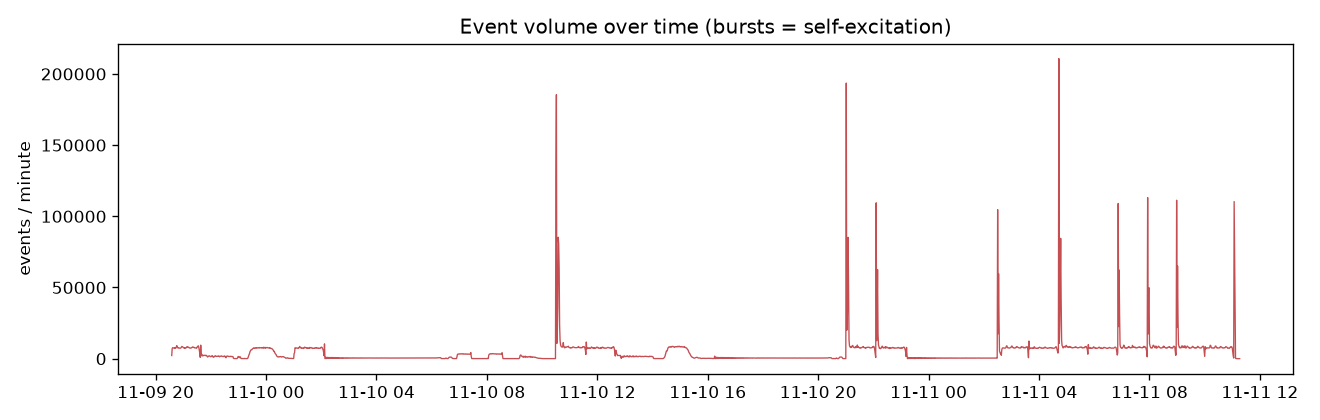
\includegraphics[width=0.49\textwidth]{HDFS_timeline.png}}{\fbox{HDFS\_timeline.png}}
\IfFileExists{figures/HDFS_block_sizes.png}{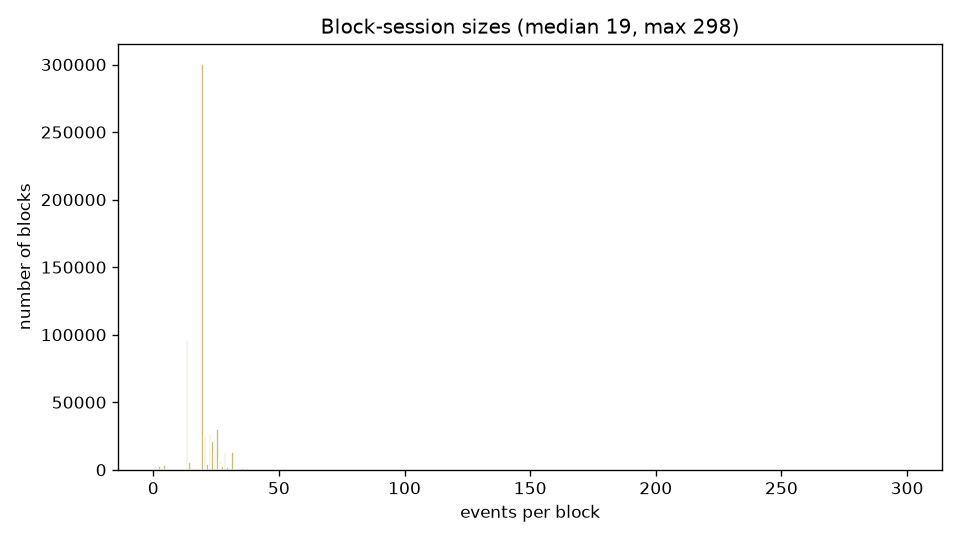
\includegraphics[width=0.49\textwidth]{HDFS_block_sizes.png}}{\fbox{HDFS\_block\_sizes.png}}
\caption{\textbf{Left:} HDFS event volume per minute---a flat baseline punctuated
by sharp bursts, the visible signature of self-excitation (Fano factor $5.3\gg1$).
\textbf{Right:} block-session sizes (median $19$, max $298$); the long tail is
disproportionately the anomalous blocks.}
\label{fig:eda}
\end{figure}

% ================================================================
\section{Detection on HDFS}
\label{sec:detect}

\subsection{The detection unit and the features}
Because HDFS labels are per block and a block lives $\leq54$\,s, the unit of
detection is the \keyword{block session}. We represent each block by a
\keyword{count vector}: a $48$-dimensional vector whose $j$-th entry is how many
times template $j$ occurred in that block (the standard ``event count matrix'').
This throws away timing (justified on HDFS, whose timing is unusable) and keeps
\emph{which} events occurred and \emph{how often}---a compact fingerprint of the
block's behaviour. There are $575{,}061$ such vectors.

\subsection{The validation protocol (the heart of the project)}
\begin{itemize}[nosep,leftmargin=1.5em]
  \item \keyword{Strict temporal split.} Blocks are ordered by their start time;
  the earliest $70\%$ ($402{,}543$ blocks) are training, the latest $30\%$
  ($172{,}518$ blocks) are test. The boundary falls at
  \code{2008-11-11 06:00:46}. Nothing from the test period touches training,
  scaling, or thresholds (Section~\ref{sec:primer-temporal}).
  \item \keyword{Train on normal only.} The autoencoder trains on the
  $389{,}428$ \emph{normal} training blocks; anomaly labels never enter training.
  \item \keyword{PR-AUC}, not accuracy or ROC (Section~\ref{sec:primer-metrics}).
  \item \keyword{False alarms per day at $90\%$ recall}, on real elapsed test
  time.
  \item \keyword{Drift}: every metric is also reported over consecutive
  chronological slices of the test window.
\end{itemize}
An honest subtlety we surface: splitting by block \emph{count} (the loglizer
convention) makes the test window time-dense---the $172{,}518$ test blocks span
only $\sim$5 hours because blocks cluster near the end---so ``per day'' is
computed from the \emph{actual} $\sim$5-hour span, not assumed uniform.

\subsection{The two models}
\begin{itemize}[nosep,leftmargin=1.5em]
  \item \textbf{Isolation Forest (baseline)}, fit on $\log(1+\text{counts})$ (the
  log tames a few very frequent templates); anomaly score $=-\,$\code{score\_samples}
  (oriented so higher $=$ more anomalous).
  \item \textbf{Autoencoder (detector)}: an MLP
  $48\!\to\!32\!\to\!16\!\to\!8\!\to\!16\!\to\!32\!\to\!48$ with ReLU
  activations, trained with Adam to minimise reconstruction MSE on normal
  training blocks, with early stopping on a held-out slice of the normal training
  data (it converged in $\sim$19 epochs). Inputs are $\log(1+\text{counts})$ then
  standardised, with the scaler fit on normal training data only. The per-block
  reconstruction MSE is the anomaly score. Both scores feed the \emph{same}
  evaluation code, so the comparison is exactly apples-to-apples.
\end{itemize}

\subsection{Results}
\begin{table}[H]
\centering
\caption{HDFS detection on the test split ($172{,}518$ blocks, $2.16\%$
anomalous).}
\label{tab:detect}
\small
\renewcommand{\arraystretch}{1.15}
\begin{tabular}{@{}l c c@{}}
\toprule
Metric & Isolation Forest & \color{good}Autoencoder \\
\midrule
PR-AUC (average precision) & $0.748$ & \ours{$0.987$} \\
Precision @ 90\% recall & $0.556$ & \ours{$0.961$} \\
False alarms / day @ 90\% recall & $\sim$$12{,}700$ & \ours{$\sim$$650$} \\
\bottomrule
\end{tabular}
\end{table}

\paragraph{Reading the numbers.} The autoencoder's PR-AUC of $0.987$ (against a
chance line of $0.022$) means it ranks almost all anomalies above almost all
normal blocks. Operationally it is decisive: at the same $90\%$ detection rate it
produces $\sim$$650$ false alarms/day versus the baseline's $\sim$$12{,}700$---a
$\sim$$20\times$ reduction. Figure~\ref{fig:pr} shows the full precision--recall
curves; the autoencoder holds near-perfect precision until $\sim$$0.95$ recall.

\begin{figure}[H]
\centering
\IfFileExists{figures/hdfs_pr_comparison.png}{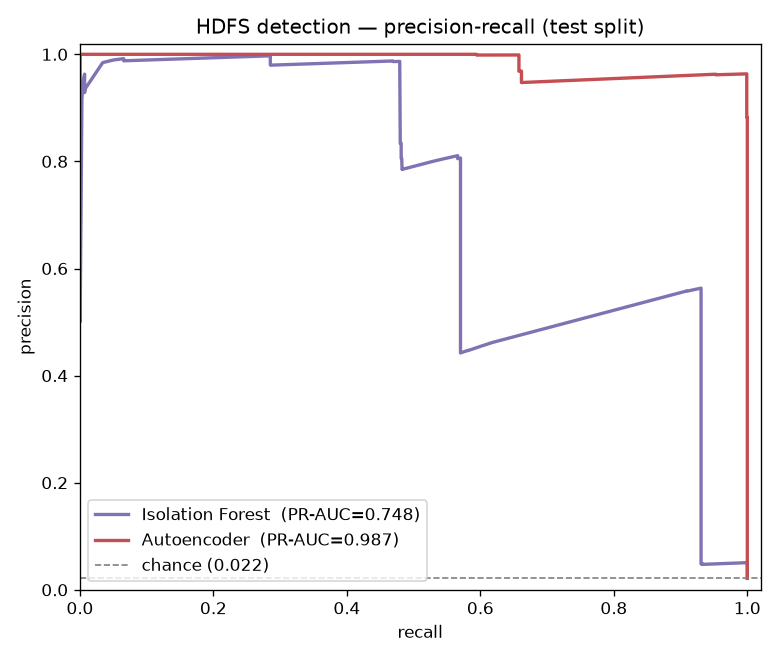
\includegraphics[width=0.62\textwidth]{hdfs_pr_comparison.png}}{\fbox{hdfs\_pr\_comparison.png}}
\caption{HDFS precision--recall, test split. The autoencoder (PR-AUC $0.987$)
dominates the Isolation Forest baseline ($0.748$) at every operating point; the
dashed line is the $0.022$ chance level.}
\label{fig:pr}
\end{figure}

\paragraph{The drift result (why this matters more than the headline).} We also
computed PR-AUC over four consecutive slices of the 5-hour test window. The
baseline's discrimination swung wildly ($0.69$--$0.98$), while the autoencoder
held $\geq0.99$ throughout. So the autoencoder is not just more accurate but more
\emph{stable}---a property invisible to a single aggregate number and exactly what
the drift check is designed to expose. Crucially, however, the \emph{false-alarm
rate} at a fixed threshold was \emph{not} stable even for the autoencoder
(it swung by orders of magnitude across the window)---the problem
Section~\ref{sec:evt} then solves.

\begin{takeaway}
The HDFS autoencoder is a strong \emph{reproduction} (PR-AUC $0.987$), used here
to validate the pipeline and feed the triage layer---not claimed as novel. Its
real lesson is the drift analysis: aggregates hide instability that only
per-period measurement reveals.
\end{takeaway}

% ================================================================
\section{The mathematical core: Hawkes process on BGL}
\label{sec:hawkes}

This is the intellectual centerpiece. We model \emph{when} BGL events happen with
a self-exciting point process, estimate how cascade-prone the system is, validate
the fit rigorously, and later test whether the model helps detection.

\subsection{The model, restated with meaning}
The exponential-kernel Hawkes intensity (Equation~\ref{eq:hawkes-primer}) is
\[
\lambda(t)=\mu+\sum_{t_i<t}\alpha\,e^{-\beta(t-t_i)}.
\]
Reading each symbol: $\mu$ is the rate of ``spontaneous'' events; $\alpha$ is how
much the intensity jumps the instant an event occurs; $\beta$ is the decay rate,
so $1/\beta$ is the characteristic time over which one event's influence fades.
The branching ratio $\eta=\alpha/\beta$ (Section~\ref{sec:primer-hawkes}) is the
mean number of direct offspring per event.

\subsection{Estimating $(\mu,\alpha,\beta)$ by maximum likelihood}
We choose the parameters that make the observed event times most probable. For a
point process observed on $[0,T]$, the log-likelihood is
\begin{equation}
\ell(\mu,\alpha,\beta)=\sum_i \log\lambda(t_i)\;-\;\int_0^T\lambda(s)\,ds.
\label{eq:ll}
\end{equation}
The two terms have clean meanings. The first \emph{rewards} placing high
intensity exactly where events actually occurred (a good model is ``surprised''
little by the real events). The second \emph{penalises} predicting a high total
number of events overall (the integral is the model's expected event count); it
stops the trivial cheat of setting the intensity huge everywhere.

For the exponential kernel both terms are cheap. The integral is closed-form,
\begin{equation}
\int_0^T\lambda(s)\,ds=\mu T+\frac{\alpha}{\beta}\sum_i\Bigl(1-e^{-\beta(T-t_i)}\Bigr),
\end{equation}
and the sum $\sum_i\log\lambda(t_i)$ is computed in \emph{linear} time using
Ogata's recursion: the excitation felt at event $i$,
$A_i=\sum_{j<i}e^{-\beta(t_i-t_j)}$, satisfies
\begin{equation}
A_i=e^{-\beta(t_i-t_{i-1})}\bigl(1+A_{i-1}\bigr),\qquad A_1=0,
\qquad \lambda(t_i)=\mu+\alpha A_i.
\end{equation}
This recursion is the reason the fit is feasible on millions of events---the naive
double sum would be quadratic. We maximise $\ell$ over $(\log\mu,\log\alpha,
\log\beta)$ (the log-parametrisation makes the positivity constraints automatic
and the optimisation unconstrained) with the L-BFGS-B optimiser.

\subsection{Correctness before trust: recovery from simulation}
A fitted number is worthless unless the fitter is correct. Because this is the
centerpiece, we \emph{proved} the implementation before touching BGL: we simulate
a Hawkes process with \emph{known} parameters using Ogata's thinning algorithm,
then fit it and check the estimates match. They do (within a few percent). We also
verified that the time-rescaling test \emph{passes} a correct fit and
\emph{rejects} a deliberately-wrong model. These checks live in
\code{tests/test\_hawkes.py} and run in the automated test suite. We implemented
everything in \code{scipy} because the standard \code{tick} library has no
installable build for modern Python; the mathematics is library-independent.

\subsection{Validating the fit with the time-rescaling theorem}
As explained in Section~\ref{sec:primer-rescaling}, if the fit is good the
rescaled inter-event gaps $\Delta\tau_i=\Lambda(t_i)-\Lambda(t_{i-1})$ are i.i.d.\
$\mathrm{Exp}(1)$. We compute them, plot them against the ideal $\mathrm{Exp}(1)$
quantiles (a QQ-plot: points on the diagonal $=$ perfect fit), and run a KS test.
A single interpretable diagnostic---the \emph{mean} rescaled gap---should be
exactly $1$ if the compensator is correct, independent of shape; we use it as a
normalisation sanity check.

\subsection{Results and interpretation}
\begin{table}[H]
\centering
\caption{Hawkes fits on two BGL windows (all events).}
\label{tab:hawkes}
\small
\renewcommand{\arraystretch}{1.15}
\begin{tabular}{@{}l c c c c@{}}
\toprule
BGL window & Events & \textbf{$\eta=\alpha/\beta$} & KS statistic & mean rescaled gap \\
\midrule
2005-09-03 (calm day) & $6{,}858$ & $\mathbf{0.971}$ & $0.095$ & $1.0001$ \\
2005-06-11 (fault cascade) & $152{,}669$ & $\mathbf{0.9998}$ & $0.431$ & $1.0000$ \\
\bottomrule
\end{tabular}
\end{table}

\paragraph{The headline: near-critical self-excitation.} On both windows the
branching ratio is $\eta\approx0.97$--$1.0$---remarkably close to the critical
value $1$. In plain terms, \emph{each BGL event triggers on the order of one
direct offspring event}: the system sits right at the edge where cascades become
self-sustaining. This is a precise, estimated, interpretable statement about the
data, far stronger than ``the logs are bursty.'' Figure~\ref{fig:hawkes} (top)
visualises the fitted intensity $\lambda(t)$: near-zero between bursts, spiking
sharply (to $\sim$$190$ events/s) as each cascade self-excites.

\paragraph{The honest caveat: where the single-exponential kernel breaks.} The
QQ-plots (Figure~\ref{fig:hawkes}, bottom) show the \emph{bulk} of the rescaled
gaps lying on the $\mathrm{Exp}(1)$ diagonal---the model captures ordinary
clustering well---but the \emph{upper tail} bending upward: the longest quiet gaps
are longer than a single exponential predicts. The mechanism is intuitive: right
after a burst the fitted excitation expects many events; when silence follows
instead, the model has ``over-predicted,'' and the integrated intensity over that
gap is large, producing an outlying rescaled gap. A single exponential cannot
simultaneously fit tight bursts and deep lulls. The effect is mild on the calm day
(KS $0.095$) and severe on the extreme cascade (KS $0.431$, with $\eta$ pinned at
the critical boundary). The mean rescaled gap of exactly $1.0000$ confirms the
compensator is correctly normalised even where the shape deviates; and because
the KS test has enormous power at $10^5$ points (it rejects essentially any
parametric model at that sample size), we judge the fit by the \emph{shape} of
the QQ-plot and the \emph{magnitude} of deviation, not by the $p$-value.

\begin{figure}[H]
\centering
\IfFileExists{figures/bgl_hawkes_2005-09-03_all_intensity.png}{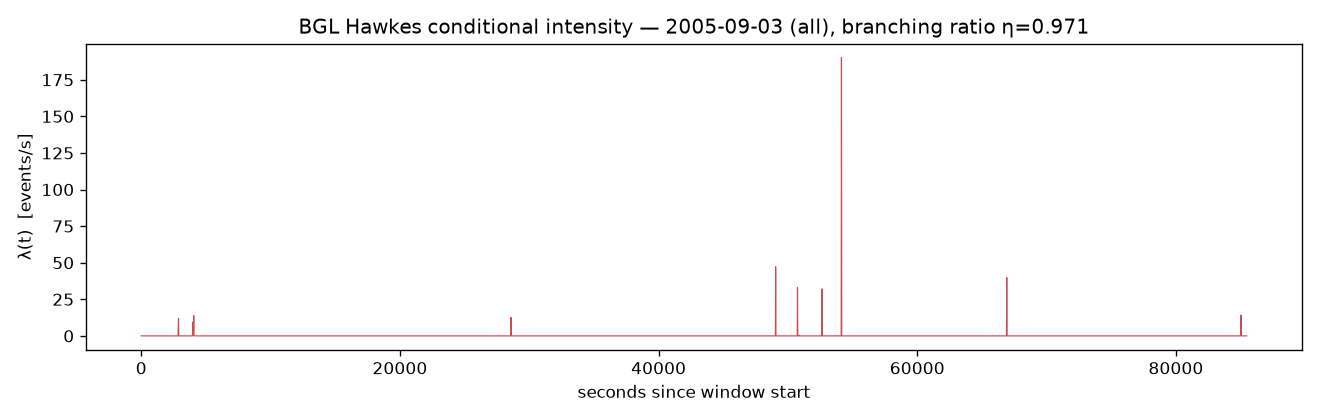
\includegraphics[width=0.72\textwidth]{bgl_hawkes_2005-09-03_all_intensity.png}}{\fbox{intensity}}\\[4pt]
\IfFileExists{figures/bgl_hawkes_2005-09-03_all_qq.png}{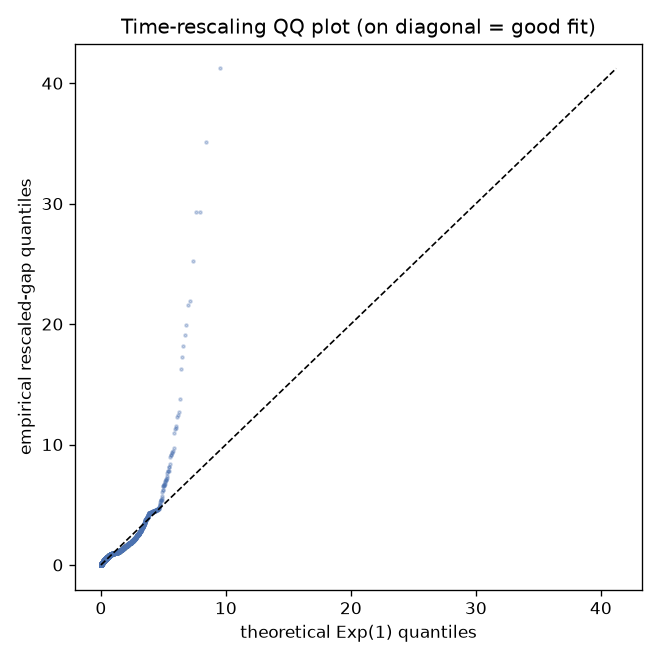
\includegraphics[width=0.40\textwidth]{bgl_hawkes_2005-09-03_all_qq.png}}{\fbox{qq calm}}
\IfFileExists{figures/bgl_hawkes_2005-06-11_all_qq.png}{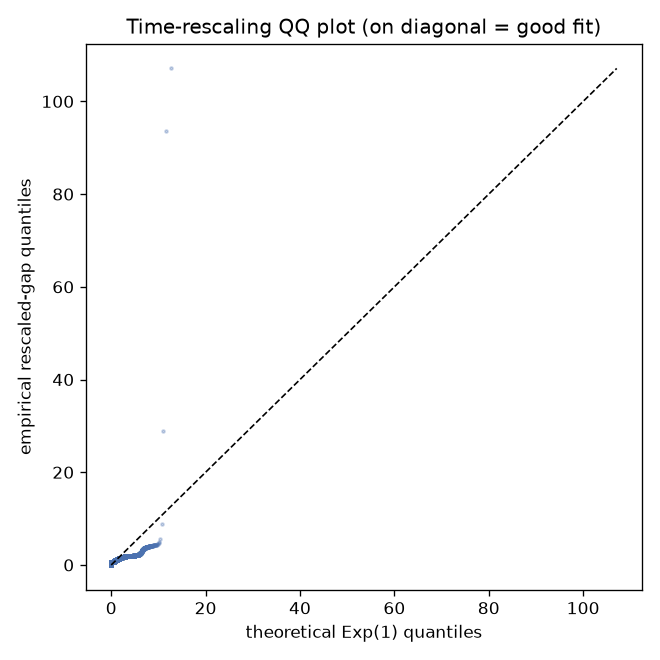
\includegraphics[width=0.40\textwidth]{bgl_hawkes_2005-06-11_all_qq.png}}{\fbox{qq cascade}}
\caption{\textbf{Top:} fitted conditional intensity $\lambda(t)$ on the calm day
---near-zero baseline with sharp self-exciting spikes. \textbf{Bottom:}
time-rescaling QQ-plots for the calm window (left, KS $0.095$) and the extreme
cascade (right, KS $0.431$). Both show the body on the ideal diagonal and the
upper tail deviating---the single-exponential kernel underfits the deepest lulls.}
\label{fig:hawkes}
\end{figure}

\begin{takeaway}
BGL's event stream is \emph{near-critically self-exciting} ($\eta\approx0.97$--
$1.0$): a concrete, validated finding. The single-exponential Hawkes captures the
bulk clustering but underfits the deepest inter-event gaps---honestly characterised
via time-rescaling, and motivating a richer kernel as future work.
\end{takeaway}

% ================================================================
\section{Does the timing signal actually help detection?}
\label{sec:ablation}

Fitting a Hawkes process is elegant, but a professional reader will ask: does it
\emph{help}? We tested this directly rather than assuming, and report the honest
answer. On fixed 60-second BGL windows we detect alert-containing windows three
ways with the \emph{same} model (Isolation Forest) and the \emph{same} temporal
split, changing \emph{only} the features:

\begin{itemize}[nosep,leftmargin=1.5em]
  \item \textbf{content} --- counts of the top-50 event templates in the window
  (which events occurred; ignores timing).
  \item \textbf{timing} --- the per-window Hawkes self-excitation
  $A(t)=\sum_{t_i<t}e^{-\beta(t-t_i)}$ summarised (mean/max) at two decay scales
  ($1$\,s and $30$\,s), plus the event count. Computed from event \emph{times
  only}---no labels---so it is a legitimate, leakage-free detector feature. High
  $A(t)$ means ``this window sits inside a self-exciting cascade.''
  \item \textbf{content+timing} --- both feature blocks concatenated.
\end{itemize}

\begin{table}[H]
\centering
\caption{BGL window detection, feature ablation (test split, $4.71\%$ anomalous).}
\label{tab:ablation}
\small
\renewcommand{\arraystretch}{1.15}
\begin{tabular}{@{}l c c c@{}}
\toprule
Feature set & PR-AUC & Precision @ 90\% recall & False alarms / day \\
\midrule
content & $0.081$ & $0.046$ & $114$ \\
\rowcolor{keybg}\color{good}timing & \color{good}$0.087$ & \color{good}$0.083$ & \color{good}$61$ \\
content+timing & $0.090$ & $0.071$ & $72$ \\
chance & $0.047$ & --- & --- \\
\bottomrule
\end{tabular}
\end{table}

\paragraph{The honest, nuanced answer.} Two things are true at once. First,
\emph{absolute detection here is weak}: all three feature sets sit around PR-AUC
$0.09$, only $\sim$$2\times$ the $0.047$ chance line. Detecting BGL fault windows
at 60-second resolution is genuinely hard---most alert windows fold a handful of
alert lines into heavy normal traffic, so the unsupervised signal is faint. We do
not oversell it. Second, and more interestingly, \emph{the timing signal is the
more useful one and it cuts false alarms}: at $90\%$ recall, timing roughly
\emph{halves} the false-alarm rate versus content ($114\!\to\!61$ per day) and
nearly doubles precision ($0.046\!\to\!0.083$). Figure~\ref{fig:ablation} shows
why: the content curve collapses to the chance line at high recall, while the
timing curve holds $\sim$$2\times$ chance across the operational range.

\begin{takeaway}
On BGL the Hawkes self-excitation feature is the single most useful signal and
roughly halves false alarms at a fixed detection rate---but it does not, alone,
turn window-level detection into a strong detector. ``Timing beats content and
halves false alarms, on a hard task'' is a real, validated result; a manufactured
$0.98$ would not be.
\end{takeaway}

\begin{figure}[H]
\centering
\IfFileExists{figures/bgl_timing_ablation.png}{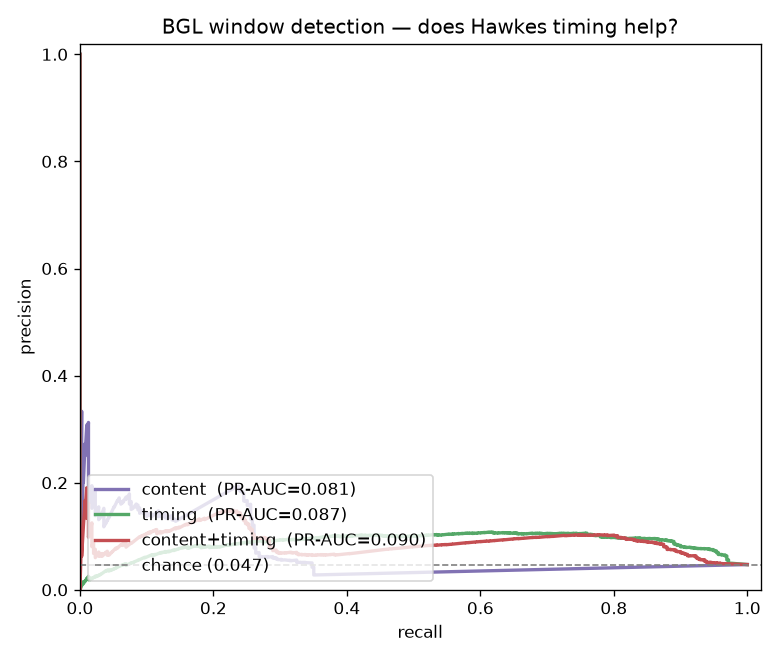
\includegraphics[width=0.58\textwidth]{bgl_timing_ablation.png}}{\fbox{bgl\_timing\_ablation.png}}
\caption{BGL window detection precision--recall. All feature sets are weak in
absolute terms, but timing (green) and content+timing (red) clearly dominate
content (purple), which collapses to the chance line at higher recall.}
\label{fig:ablation}
\end{figure}

% ================================================================
\section{Adaptive thresholding: stabilising false alarms under drift}
\label{sec:evt}

\subsection{The problem, made concrete}
A detector produces a continuous score; a \emph{threshold} turns it into alerts.
The drift analysis (Section~\ref{sec:detect}) exposed the real operational
weakness: at a \emph{fixed} threshold, the false-alarm rate wanders as the score
distribution drifts, even while ranking quality (PR-AUC) stays high. Measured on
the HDFS autoencoder scores across the 5-hour test window, a fixed threshold's
false alarms swing from $3{,}664$ to $\mathbf{861{,}686}$ per day---at the worst
moments it flags essentially every block (Figure~\ref{fig:evt}). No analyst can
work with a false-alarm rate that varies by two orders of magnitude.

\subsection{Extreme-Value Theory: the principled tool (derivation)}
We want a threshold $z_q$ exceeded by only a small target fraction $q$ of scores
(e.g.\ $q=0.03$), \emph{recomputed as the distribution drifts}. EVT
(Section~\ref{sec:primer-evt}) says: pick a high pilot threshold $t$ (e.g.\ the
$95$th percentile); the exceedances $X-t$ above it follow a Generalized Pareto
Distribution with shape $\gamma$ and scale $\sigma$,
\begin{equation}
\Pr(X-t>x\mid X>t)\approx\Bigl(1+\tfrac{\gamma x}{\sigma}\Bigr)^{-1/\gamma}.
\end{equation}
Fit $(\gamma,\sigma)$ to the observed exceedances (we use a fast method-of-moments
estimator so it can update in $O(1)$ per new point). Then set the total tail
probability equal to the target, $\Pr(X>z_q)=(N_t/n)\,(1+\gamma(z_q-t)/\sigma)^{-1/\gamma}=q$,
and solve for the threshold:
\begin{equation}
z_q=t+\frac{\sigma}{\gamma}\!\left[\Bigl(\frac{q\,n}{N_t}\Bigr)^{-\gamma}-1\right],
\end{equation}
with $n$ the sample size and $N_t$ the number of exceedances above $t$. Holding
$q$ fixed while re-estimating $(t,\gamma,\sigma)$ on a trailing window keeps the
flagged fraction---hence the false-alarm rate---steady as the scores drift. We
implemented this (\code{AdaptivePot}) and verified on simulated data that it
controls the exceedance rate and tracks drift where a fixed threshold fails.

\subsection{An honest negative finding, and the fix}
When we applied EVT to the HDFS autoencoder scores it \emph{misbehaved}: the fitted
threshold sometimes fell below the data floor and flagged everything. The cause is
real and instructive. The autoencoder scores are strongly \emph{discrete}:
$58.7\%$ of normal blocks reconstruct to the \emph{identical} value, because normal
HDFS blocks are so repetitive that huge groups have byte-identical count vectors.
GPD assumes a \emph{continuous} tail; a distribution with a giant point mass
violates that assumption, and the extrapolation breaks. So we did the honest
thing: on HDFS we use the distribution-free \keyword{rolling quantile} (the
empirical $(1-q)$-quantile of a trailing window, which makes no distributional
assumption), and we reserve EVT for BGL's genuinely continuous timing scores,
where its extrapolation to small $q$ earns its place.

\subsection{Result}
\begin{table}[H]
\centering
\caption{HDFS false-alarm stability under drift (autoencoder scores, target flag
rate $q=3\%$).}
\label{tab:evt}
\small
\renewcommand{\arraystretch}{1.15}
\begin{tabular}{@{}l c c@{}}
\toprule
 & Fixed threshold & \color{good}Adaptive (rolling quantile) \\
\midrule
False alarms / day (range over test) & $3{,}664$--$861{,}686$ & \ours{$0$--$7{,}584$} \\
Flagged fraction & up to $100\%$ & \ours{stable $\approx2\%$} \\
Recall & $1.00$ & $0.72$ \\
\bottomrule
\end{tabular}
\end{table}

The adaptive threshold rises and falls to track the drifting scores, holding the
alert rate near target instead of exploding (Figure~\ref{fig:evt}). The
transparent cost is recall: in periods where anomalies surge past the flag budget,
holding the false-alarm rate constant means catching fewer of them
($1.00\!\to\!0.72$). This is the true operating-point tradeoff, now made
\emph{explicit and tunable} via the single knob $q$, rather than hidden.

\begin{figure}[H]
\centering
\IfFileExists{figures/hdfs_evt_thresholding.png}{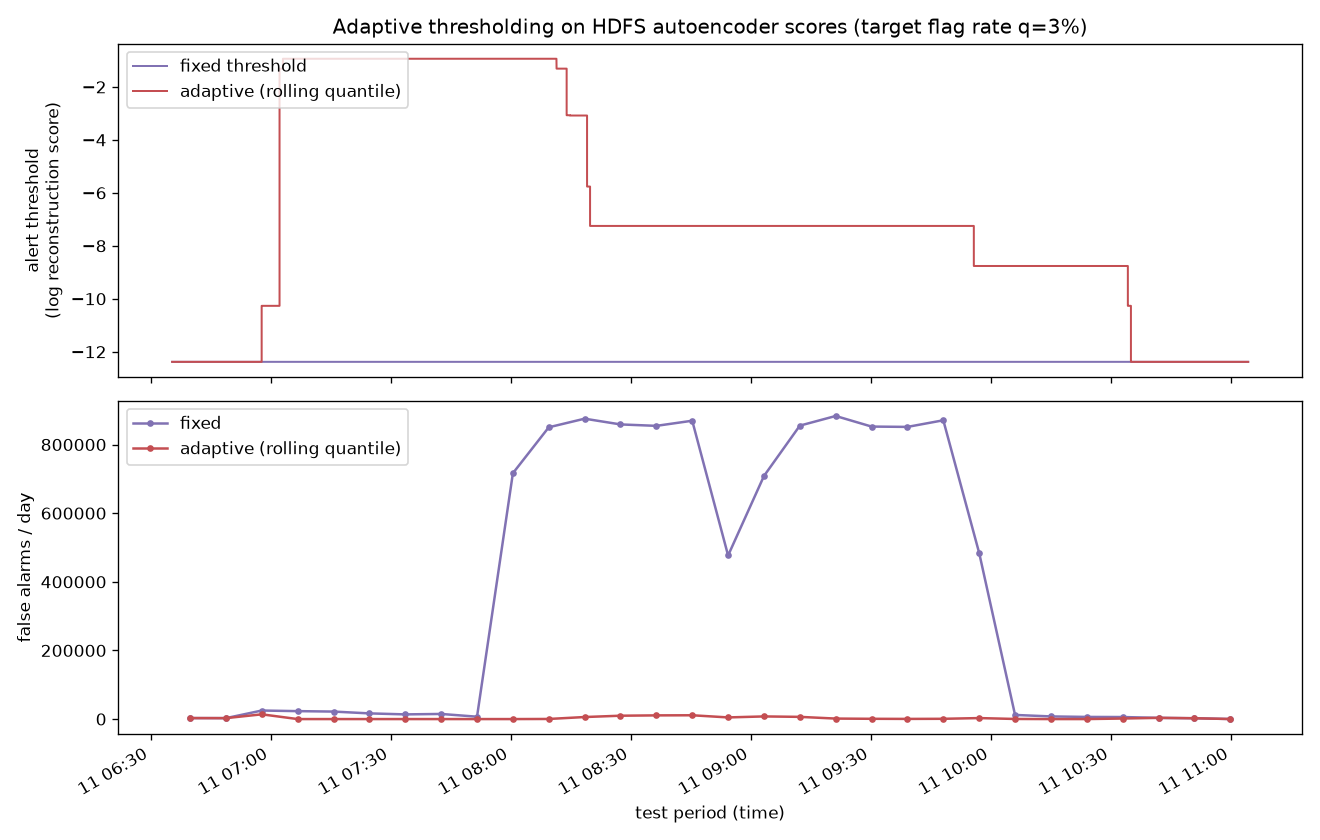
\includegraphics[width=0.80\textwidth]{hdfs_evt_thresholding.png}}{\fbox{hdfs\_evt\_thresholding.png}}
\caption{\textbf{Top:} the fixed threshold stays put while the normal-block scores
drift upward mid-period; the adaptive threshold rises to track them.
\textbf{Bottom:} the fixed threshold's false alarms explode to $\sim$860k/day
mid-period; the adaptive threshold holds the alert rate near target throughout.}
\label{fig:evt}
\end{figure}

\begin{takeaway}
A fixed threshold is undeployable under drift---the false-alarm rate is what moves,
and it moves by $\sim$$235\times$. A trailing-window adaptive threshold stabilises
it at a transparent, tunable recall cost. EVT is the right tool for continuous
scores; HDFS's discrete scores require the distribution-free rolling quantile
instead---a finding we report rather than paper over.
\end{takeaway}

% ================================================================
\section{LLM triage: from raw alerts to ranked incidents}
\label{sec:triage}

Detection produces many flagged units; paging an analyst once per flag is
unusable. The triage agent reduces volume, then explains, in three steps.

\begin{enumerate}[leftmargin=1.6em]
  \item \keyword{Deduplicate.} Flags with the same \emph{signature}---same entity
  (block/node) and same multiset of event templates---collapse into a single
  representative, carrying a count. Identical repeated alerts are recorded once,
  not re-paged.
  \item \keyword{Correlate into incidents.} Flags close together in time are
  grouped into one \emph{incident}. This is the Hawkes idea made
  operational: self-exciting events are causally linked, so a temporal cascade of
  anomalies is \emph{one} root-cause incident, not two hundred separate pages.
  This grounding in the timing model is what distinguishes it from an arbitrary
  fixed-window heuristic.
  \item \keyword{Explain and rank.} Each incident is classified into
  strictly-typed JSON---\code{priority}, \code{category}, \code{summary},
  \code{recommended\_action}, \code{explanation}---and the incidents are ranked
  P1$\to$P4 by priority then peak score. The explainer is \emph{pluggable}: a
  deterministic rule-based backend (category from template keywords; priority from
  severity and cascade size) runs fully self-contained, while an \keyword{Anthropic
  backend} (\code{claude-opus-4-8}, using \emph{structured outputs} so the model
  is forced to return exactly the required JSON schema) drops in when an API key is
  configured, and falls back automatically if not. There is one model call per
  \emph{incident}, not per raw flag---the dedup/correlation makes the LLM cost
  scale with incidents, not alerts.
\end{enumerate}

\paragraph{Result.} On the top-200 flagged HDFS blocks, the agent produced
\textbf{200 raw flags $\to$ 90 incidents}, ranked P1(13) / P2(53) / P3(2) /
P4(22) across \emph{data-loss}, \emph{replication-failure}, and \emph{network}
categories (Figure~\ref{fig:dash}). An operator sees $90$ prioritised, explained
incidents instead of $200$ undifferentiated alerts.

\begin{takeaway}
Triage turns a flood of flags into a short, ranked, explained incident list. Its
one conceptual novelty is that correlation is grounded in the same self-excitation
model as the rest of the project: a cascade is one incident.
\end{takeaway}

\paragraph{Honest note on the LLM backend.} This build environment has no model
credential, so the demonstration ran on the deterministic rule-based explainer.
The Anthropic path is written against the current API (structured outputs,
\code{claude-opus-4-8}) and activates with a key; it was not exercised live here.

% ================================================================
\section{The dashboard and software architecture}
\label{sec:dashboard}

\paragraph{Dashboard.} A Streamlit application (\code{app/dashboard.py}) presents
the whole pipeline in four tabs---Detection (metrics + PR curve), Thresholding (the
drift-stabilisation plot), Hawkes (intensity + QQ), and Incidents (the ranked
table with per-incident drill-down showing summary, action, and explanation). It
was verified to start and render headless (Figure~\ref{fig:dash}); ``logs in,
ranked and explained incidents out.''

\begin{figure}[H]
\centering
\IfFileExists{figures/dashboard_incidents.png}{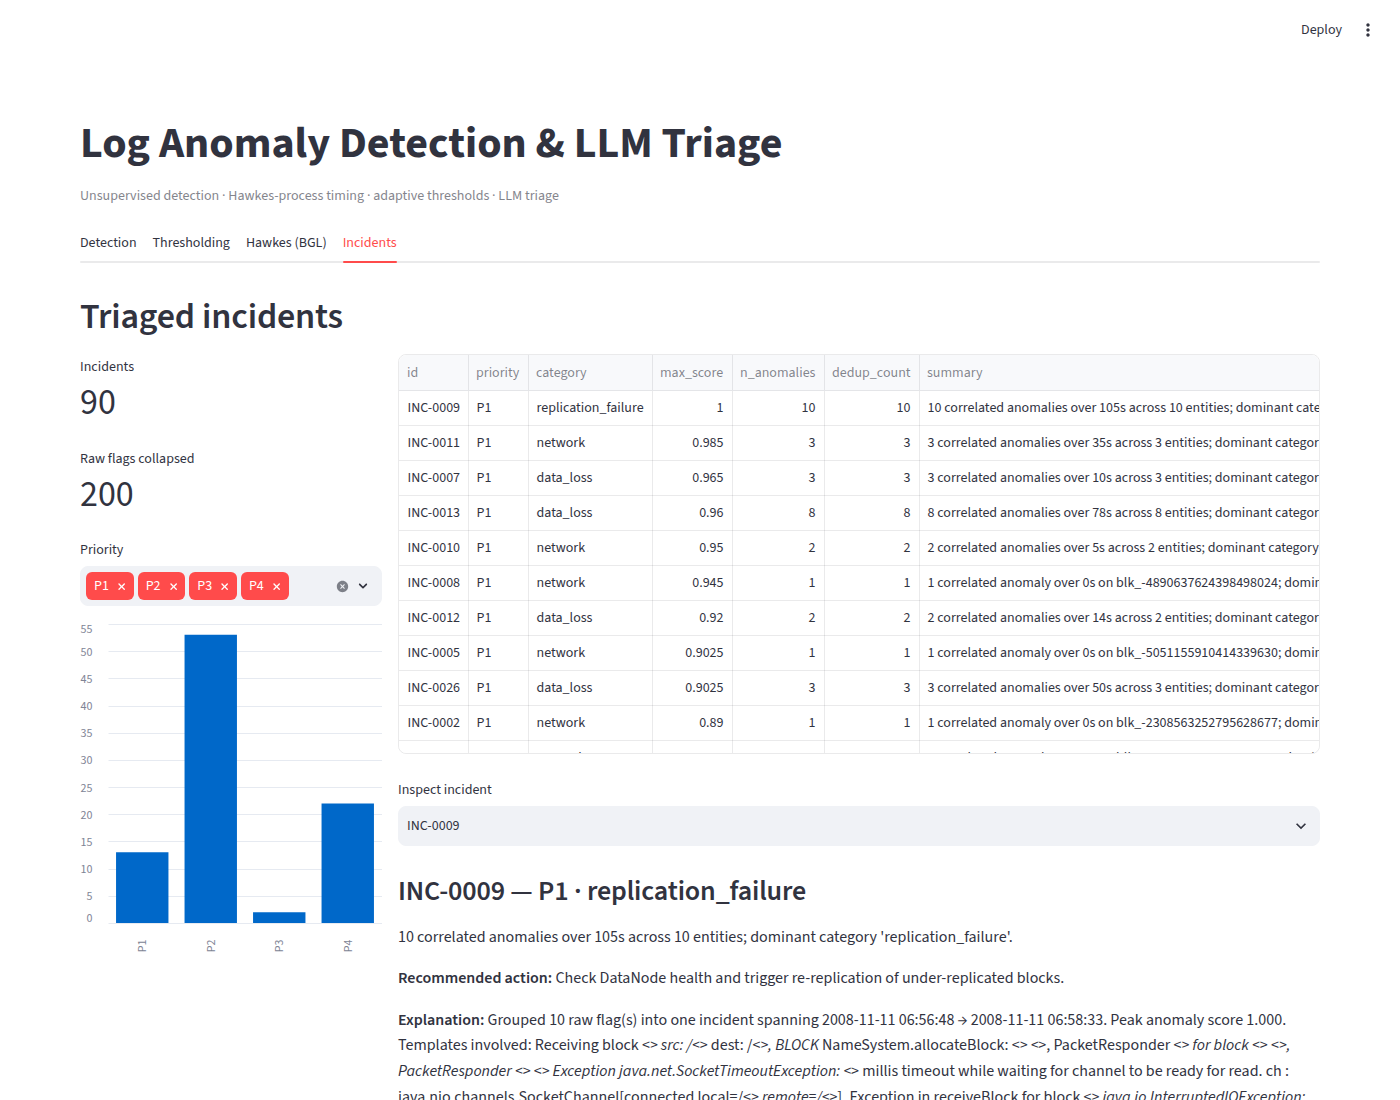
\includegraphics[width=0.82\textwidth]{dashboard_incidents.png}}{\fbox{dashboard\_incidents.png}}
\caption{The dashboard's Incidents tab: $200$ raw flags collapsed to $90$ ranked
incidents, with the priority distribution and a per-incident drill-down.}
\label{fig:dash}
\end{figure}

\paragraph{Software architecture.} The code is a small installable Python package,
\code{src/logtriage/}, with one sub-module per pipeline stage---\code{data}
(download/load), \code{parsing} (Drain wrapper), \code{features} (block-session
and window features), \code{models} (Isolation Forest, autoencoder), \code{hawkes}
(intensity, MLE, simulation, time-rescaling), \code{eval} (PR-AUC, false-alarms-
per-day, drift, EVT), and \code{triage} (incident model, explainers, agent). Thin
scripts in \code{scripts/} are the runnable entry points, one per stage, each
reading the previous stage's output from \code{data/}. This keeps logic testable
and reused identically by scripts, notebooks, and the dashboard.
\textbf{34 unit tests} cover the load-bearing logic---parameter recovery for the
Hawkes fitter, the metric definitions, the EVT rate control, the triage
correlation, and more---so a regression is caught immediately.

% ================================================================
\section{Results at a glance}
\label{sec:results}

\begin{table}[H]
\centering
\caption{Consolidated results.}
\small
\renewcommand{\arraystretch}{1.2}
\begin{tabular}{@{}l l@{}}
\toprule
Result & Value \\
\midrule
HDFS parsed & 11.2M lines $\to$ 48 templates \\
BGL parsed & 4.71M lines $\to$ 429 templates \\
Autoencoder PR-AUC (test) & \ours{$0.987$} \; (baseline $0.748$) \\
False alarms/day @ 90\% recall & \ours{$\sim$$650$} \; (baseline $\sim$$12{,}700$) \\
Hawkes branching ratio (BGL) & \ours{$\eta\approx0.97$--$1.0$} (near-critical) \\
Timing feature effect (BGL) & \ours{halves} false alarms vs.\ content \\
Fixed $\to$ adaptive threshold & FA/day swing $\times235 \to$ held near target \\
Triage reduction & 200 flags $\to$ \ours{90 ranked incidents} \\
Unit tests & \textbf{34 passing} \\
\bottomrule
\end{tabular}
\end{table}

% ================================================================
\section{Honest limitations}
\label{sec:limits}
\begin{itemize}[nosep,leftmargin=1.5em]
  \item \textbf{HDFS detection is a reproduction}, not a contribution; its role is
  validation and substrate, stated plainly.
  \item \textbf{BGL window detection is weak in absolute terms} ($\sim$$0.09$
  PR-AUC); the timing result is a \emph{relative} win (fewer false alarms) on a
  hard task, not a strong detector.
  \item \textbf{The single-exponential Hawkes kernel underfits} BGL's deepest lulls
  (the time-rescaling upper tail); a sum-of-exponentials or power-law kernel is the
  natural fix.
  \item \textbf{EVT does not fit the discrete HDFS scores}; the rolling quantile is
  used there, and EVT is reserved for continuous scores.
  \item \textbf{The LLM triage backend was not exercised live} (no credential in
  this environment); only the rule-based path ran end-to-end.
  \item \textbf{Hyperparameters are first choices, not swept}: window size
  ($60$\,s), the top-50 template vocabulary, the two decay scales, and the network
  architecture were reasonable defaults, not tuned on a validation set.
\end{itemize}

% ================================================================
\section{Conclusion and future work}
\label{sec:conclusion}
We built a complete, unsupervised log-anomaly pipeline with a stochastic-process
core and an LLM triage layer, validated with a discipline---temporal split,
PR-AUC, false-alarms-per-day, and drift---that most public reproductions skip. The
mathematical centerpiece, a Hawkes process fit and validated on BGL, yields a
concrete interpretable finding (a near-critical branching ratio) and an honest
account of where a single-exponential kernel breaks. The timing signal it produces
measurably reduces false alarms even though absolute detection on BGL is hard.
Throughout, we separated what the community has already established from what we
contributed, and treated negative and nuanced results as first-class outcomes.

\paragraph{Future work.} (1) A richer Hawkes kernel (sum-of-exponentials /
power-law) to fix the upper-tail misfit revealed by time-rescaling. (2) Use the
time-rescaling \emph{residual} directly as a calibrated timing-anomaly detector,
with EVT thresholding on those continuous scores. (3) Sweep window size and decay
scales, and try the autoencoder in place of Isolation Forest for the timing
ablation. (4) Exercise the LLM triage end-to-end with a live model and evaluate
incident quality against held-out labels.

% ================================================================
\appendix
\section{Notation}
\begin{table}[H]\centering\small
\renewcommand{\arraystretch}{1.15}
\begin{tabular}{@{}c l@{}}
\toprule
Symbol & Meaning \\
\midrule
$\lambda(t)$ & conditional intensity: instantaneous event rate given the past \\
$\mu$ & Hawkes background (spontaneous) rate \\
$\alpha$ & Hawkes excitation jump per event \\
$\beta$ & Hawkes decay rate ($1/\beta$ = influence timescale) \\
$\eta=\alpha/\beta$ & branching ratio: mean direct offspring per event \\
$\Lambda(t)=\int_0^t\lambda$ & compensator (expected event count by time $t$) \\
$\Delta\tau_i$ & rescaled inter-event gap ($\mathrm{Exp}(1)$ under a correct fit) \\
$q$ & target tail / flagged probability for the alert threshold \\
$(\gamma,\sigma)$ & GPD shape and scale parameters (EVT tail) \\
TP,FP,FN,TN & true/false positive/negative counts \\
\bottomrule
\end{tabular}
\end{table}

\section{Glossary}
\begin{description}[leftmargin=0pt,style=nextline,itemsep=1pt]
\item[Log template / event type] The fixed ``shape'' of a family of log lines with
variable parts blanked out; produced by Drain.
\item[Block session (HDFS)] All log lines belonging to one HDFS block; the unit
that carries a label and is scored.
\item[Count vector] A window/block represented by how many times each template
occurred---the detector's input.
\item[Autoencoder] A neural network trained to reconstruct its input through a
bottleneck; reconstruction error is the anomaly score.
\item[Isolation Forest] An unsupervised detector that scores points by how few
random splits isolate them.
\item[Precision / Recall] Fraction of alerts that are real / fraction of real
anomalies caught.
\item[PR-AUC] Area under the precision--recall curve; the imbalance-robust ranking
metric.
\item[Temporal split] Train on the earlier stream, test on the strictly later
stream, never shuffled.
\item[Point process] A random model of when events occur, described by its
intensity $\lambda(t)$.
\item[Hawkes process] A self-exciting point process: each event raises the
intensity, decaying over time.
\item[Branching ratio] $\eta=\alpha/\beta$; mean direct offspring per event;
$<1$ stable, $>1$ explosive.
\item[Time-rescaling theorem] A goodness-of-fit test: under a correct fit the
rescaled gaps are $\mathrm{Exp}(1)$.
\item[EVT / POT / GPD] Extreme-Value Theory / Peaks-Over-Threshold / Generalized
Pareto Distribution; the machinery for a self-calibrating tail threshold.
\item[Drift] Change over time in the data or score distribution; measured
per-period, not just in aggregate.
\end{description}

% ================================================================
\begin{thebibliography}{9}
\small
\bibitem{drain} P.~He, J.~Zhu, Z.~Zheng, M.~R.~Lyu. ``Drain: An Online Log Parsing
Approach with Fixed Depth Tree.'' \emph{IEEE ICWS}, 2017.
\bibitem{loglizer} S.~He, J.~Zhu, P.~He, M.~R.~Lyu. ``Experience Report: System
Log Analysis for Anomaly Detection.'' \emph{IEEE ISSRE}, 2016.
\bibitem{deeplog} M.~Du, F.~Li, G.~Zheng, V.~Srikumar. ``DeepLog: Anomaly
Detection and Diagnosis from System Logs through Deep Learning.'' \emph{ACM CCS},
2017.
\bibitem{loganomaly} W.~Meng et al. ``LogAnomaly: Unsupervised Detection of
Sequential and Quantitative Anomalies in Unstructured Logs.'' \emph{IJCAI}, 2019.
\bibitem{hawkes} A.~G.~Hawkes. ``Spectra of Some Self-Exciting and Mutually
Exciting Point Processes.'' \emph{Biometrika}, 1971.
\bibitem{ogata} Y.~Ogata. ``On Lewis' Simulation Method for Point Processes.''
\emph{IEEE Trans.\ Information Theory}, 1981.
\bibitem{timerescaling} E.~N.~Brown, R.~Barbieri, V.~Ventura, R.~E.~Kass,
L.~M.~Frank. ``The Time-Rescaling Theorem and Its Application to Neural Spike Train
Data Analysis.'' \emph{Neural Computation}, 2002.
\bibitem{spot} A.~Siffer, P.-A.~Fouque, A.~Termier, C.~Largou\"et. ``Anomaly
Detection in Streams with Extreme Value Theory.'' \emph{ACM KDD}, 2017.
\bibitem{loghub} S.~He, J.~Zhu, P.~He, M.~R.~Lyu. ``Loghub: A Large Collection of
System Log Datasets for AI-driven Log Analytics.'' \emph{IEEE ISSRE}, 2023.
\end{thebibliography}

\end{document}
